% Master's thesis defense: MicroRTS DRL agent (UCLouvain / EPL)
% Target: ~19 min calm delivery + 10 min Q&A.
% Style: ~21 content slides, each one coherent idea worth ~50-60s of speech.
% Theme: metropolis. Compile: latexmk -pdf main.tex (needs `metropolis`).
%
% Figures: dissertation PDFs are recolored so their white background matches
% the metropolis canvas (#FAFAFA) and blends in (no white box). Recolored
% rasters live in defense/figures/<name>_bg.png (near-white >=248 -> #FAFAFA,
% 400 dpi). Photos (starcraft2, warcraft3, microRTS-image) are NOT recolored.
% To add/refresh a figure, re-run that recolor step (see defense/PLAN.md).
% If the slide background color ever changes, regenerate the _bg.png set.
% Exact numbers: defense/notes/backbone.md.

\documentclass[aspectratio=169,11pt]{beamer}

\usepackage[T1]{fontenc}
\usepackage[utf8]{inputenc}

\usetheme{metropolis}
\usepackage{appendixnumberbeamer}
\usepackage{booktabs}
\usepackage{graphicx}
\usepackage{tikz}
\usetikzlibrary{positioning, arrows.meta, fit, backgrounds, shadows}
\usepackage[most]{tcolorbox}
\usepackage{colortbl}
\usepackage{fontawesome5}

% --- Custom palette ---
\definecolor{uclBlue}{HTML}{1F3A5F}
\definecolor{uclAccent}{HTML}{E07A2F}
\definecolor{canvasbg}{HTML}{FAFAFA}
\setbeamercolor{frametitle}{bg=uclBlue}
\setbeamercolor{progress bar}{fg=uclAccent}
\setbeamercolor{alerted text}{fg=uclAccent}
\metroset{block=fill, sectionpage=none, numbering=fraction}

% Official-colour UCLouvain logo on a small white chip, top-right of each
% content slide's title bar (so the brand colours are preserved on the dark bar).
\addtobeamertemplate{frametitle}{}{%
  \begin{tikzpicture}[remember picture,overlay]
    \node[anchor=east,inner sep=1.6pt,fill=white,rounded corners=1.5pt]
      at ([xshift=-0.32cm,yshift=-0.057\paperheight]current page.north east)
      {
\includegraphics[height=0.40cm]{ucl_epl_tight.png}};
  \end{tikzpicture}%
}

% --- Dark section-transition slides: plan reminder + N/total progress bar ---
\definecolor{mStandout}{HTML}{23373B} % metropolis standout grey (matches Thank-you)
\setbeamercolor{section in toc}{fg=uclAccent}
\setbeamerfont{section in toc}{series=\bfseries}
\setbeamercolor{section in toc shaded}{fg=white!38}
\setbeamerfont{section in toc shaded}{series=\mdseries}
\newcommand{\totalparts}{10}
% Transition-slide plan entry: number + title + slide range (right), current in orange.
\newcommand{\planentry}[3]{% num, title, slide-range
  \hyperlink{part:#1}{%
  \ifnum\insertsectionnumber=#1\relax
    {\color{uclAccent}\bfseries #1.~#2\hfill {\scriptsize #3}}%
  \else
    {\color{white!45}#1.~#2\hfill {\scriptsize #3}}%
  \fi}\\[0.32em]}
\newlength{\thankwidth} % width of the closing "Thank you" (to match the orange rule)
\AtBeginSection[]{%
  {%
  \setbeamertemplate{footline}{}%
  \setbeamercolor{background canvas}{bg=mStandout}%
  \begin{frame}[plain,noframenumbering]
    \color{white}%
    \hypertarget{part:\insertsectionnumber}{}%
    \vfill
    \begin{columns}[T]
      \begin{column}{0.44\textwidth}
        {\normalsize\color{white!65}Part~{\color{uclAccent}\insertsectionnumber}~/~\totalparts}\\[1.4em]
        {\huge\bfseries\insertsectionhead\par}
      \end{column}
      \begin{column}{0.52\textwidth}
        \footnotesize
        \planentry{1}{Context \& Objective}{1--6}%
        \planentry{2}{Background}{7--11}%
        \planentry{3}{State of the Art}{12--15}%
        \planentry{4}{Contributions}{16--17}%
        \planentry{5}{Evaluation Framework}{18--21}%
        \planentry{6}{Environment Stack}{22--25}%
        \planentry{7}{The UECD Architecture}{26--31}%
        \planentry{8}{Training Recipe}{32--34}%
        \planentry{9}{Results \& Interpretation}{35--51}%
        \planentry{10}{Discussion \& Conclusion}{52--55}%
      \end{column}
    \end{columns}
    \vfill
    {\color{uclAccent}\rule{\dimexpr\insertsectionnumber\linewidth/\totalparts\relax}{2.5pt}}%
    {\color{white!22}\rule{\dimexpr\linewidth-\insertsectionnumber\linewidth/\totalparts\relax}{2.5pt}}%
  \end{frame}%
  }%
}

% Sober footer: a thin rule + muted text (name | current section | page).
% Deliberately much lighter than the blue title bar, to balance without weight.
\setbeamercolor{footbar}{fg=uclBlue!85,bg=uclBlue!6}
\setbeamertemplate{footline}{%
  \hbox{\color{uclBlue!18}\vrule width\paperwidth height0.4pt depth0pt}%
  \begin{beamercolorbox}[wd=\paperwidth,sep=0pt]{footbar}%
    \parbox[c][6ex][c]{\paperwidth}{%
      \hbox to\paperwidth{\hskip0.5cm\scriptsize\bfseries
        Mathis Delsart\hfill
        \ifnum\value{section}>0 Part~\insertsectionnumber\ --\ \insertsectionhead\fi\hfill
        \insertframenumber\,/\,\inserttotalframenumber%
        \hskip0.5cm}%
    }%
  \end{beamercolorbox}%
}

% --- Reuse the dissertation figures (vector PDFs) in place ---
\graphicspath{%
  {../figures/}%
  {../../dissertation/chapters/02_microrts_decision_problem/figures/}%
  {../../dissertation/chapters/03_reinforcement_learning/figures/}%
  {../../dissertation/chapters/04_classical_approaches_rts/figures/}%
  {../../dissertation/chapters/05_deep_rl_approaches_rts/figures/}%
  {../../dissertation/chapters/06_evaluation_framework/figures/}%
  {../../dissertation/chapters/07_env_stack/figures/}%
  {../../dissertation/chapters/08_architectures/figures/}%
  {../../dissertation/chapters/09_training_system/figures/}%
  {../../dissertation/chapters/10_results/figures/}%
  {../../dissertation/chapters/10_results/figures/multi-maps/}%
  {../../dissertation/chapters/13_future_work/figures/}%
  {../../dissertation/chapters/appendix/figures/}%
}

% Helper: a figure that never overflows the frame.
\newcommand{\fitfig}[2][0.7\textheight]{\centering\includegraphics[width=\linewidth,height=#1,keepaspectratio]{#2}}
% Text-mode bullet separator.
\newcommand{\sep}{\enskip\textperiodcentered\enskip}
% Slightly emphasized separator for the title page (blue, like the title bar).
\newcommand{\tsep}{\enskip{\footnotesize\color{uclBlue}\textbullet}\enskip}
% Numbered card (badge + heading + body), e.g. for the three reasoning axes.
\newtcolorbox{axisbox}{enhanced,nobeforeafter,width=\linewidth,height=4.7cm,valign=center,
  colback=uclBlue!4,colframe=uclBlue!20,boxrule=0.8pt,arc=7pt,left=8pt,right=8pt,top=8pt,bottom=8pt,
  drop fuzzy shadow=uclBlue!12}
\newcommand{\axisnum}[1]{\tikz[baseline=-0.62ex]\node[circle,fill=uclAccent,text=white,%
  font=\bfseries\small,inner sep=0pt,minimum size=1.55em]{#1};}
% Round icon badge (FontAwesome glyph on a coloured disc) for feature lists.
\newcommand{\chip}[1]{\tikz[baseline=-0.9ex]\node[circle,fill=uclBlue,text=white,%
  inner sep=0pt,minimum size=2.2em]{\large#1};}
% Smaller chip variant (more vertical air in long icon lists).
\newcommand{\schip}[1]{\tikz[baseline=-0.9ex]\node[circle,fill=uclBlue,text=white,%
  inner sep=0pt,minimum size=1.7em]{\normalsize#1};}
% Big chip variant: spans a two-line label+gloss block (vertically centered).
\newcommand{\bigchip}[1]{\tikz[baseline={(current bounding box.center)}]\node[circle,fill=uclBlue,text=white,%
  inner sep=0pt,minimum size=2.9em]{\LARGE#1};}
\newlength{\glosshang}
\newlength{\chipw}
% Contribution row: numbered icon chip + title + one-line gloss (no box).
\newcommand{\contrib}[4]{% icon, num, title, gloss
  \chip{#1} & {\color{uclBlue}\bfseries #2.}\ \textbf{#3}\newline
    {\footnotesize\color{black!55}#4}}
% MDP-style variant: title then a tight, smaller grey arrow sub-line.
\newcommand{\contribm}[4]{% icon, num, title, gloss
  \chip{#1} & {\color{uclBlue}\bfseries #2.}\ \textbf{#3}\par\vspace{-0.5em}
    {\scriptsize\color{black!55}$\rightarrow$ #4}}
% Colour-coded inline highlights for the title: method / domain / contributions.
\definecolor{hlTeal}{HTML}{1F8A80}
\definecolor{hlBlueT}{HTML}{2D6CB0}
% UECD figure-matching highlight colours (Entity = green, self-attention = red).
\definecolor{uecdGreen}{HTML}{33A968}
\definecolor{uecdRed}{HTML}{D0473A}
\newtcbox{\hlA}{on line,nobeforeafter,boxrule=0pt,boxsep=0pt,left=3pt,right=3pt,%
  top=1.5pt,bottom=1.5pt,arc=3pt,colback=hlTeal!18,coltext=hlTeal!80!black}
\newtcbox{\hlB}{on line,nobeforeafter,boxrule=0pt,boxsep=0pt,left=3pt,right=3pt,%
  top=1.5pt,bottom=1.5pt,arc=3pt,colback=uclAccent!22,coltext=uclAccent!85!black}
\newtcbox{\hlC}{on line,nobeforeafter,boxrule=0pt,boxsep=0pt,left=3pt,right=3pt,%
  top=1.5pt,bottom=1.5pt,arc=3pt,colback=hlBlueT!18,coltext=hlBlueT!92!black}
% Category pill (e.g. RQ tags "DESIGN" / "BUDGET").
\newtcbox{\rqtag}{on line,nobeforeafter,boxrule=0pt,boxsep=0pt,left=6pt,right=6pt,%
  top=2.5pt,bottom=2.5pt,arc=4pt,colback=black!50,coltext=white,fontupper=\small\bfseries}

\begin{document}

% =====================================================================
% TITLE PAGE (custom, decluttered, large logos)
% =====================================================================
{\setbeamertemplate{footline}{}
\begin{frame}[plain,noframenumbering]
  \begin{columns}[c]
    \begin{column}{0.62\textwidth}
      \raggedright
\includegraphics[height=1.7cm,keepaspectratio]{logo_uclouvain_bg.png}
    \end{column}
    \begin{column}{0.38\textwidth}
      \raggedleft
\includegraphics[height=1.7cm,keepaspectratio]{logo_epl_bg.png}
    \end{column}
  \end{columns}

  \vfill
  \begin{center}
    {\huge\bfseries\color{uclBlue} Deep Reinforcement Learning\\[0.2em]
     for Competitive Agents in MicroRTS\par}
    \vspace{0.55em}
    {\large\itshape\color{black!55} Architecture, Training, and Tournament Evaluation\par}
  \end{center}
  \vfill

  \begin{columns}[T]
    \begin{column}{0.5\textwidth}
      \footnotesize\color{black!75}
      Master's thesis \tsep June 23, 2026\\[0.3em]
      Master [120] in Computer Science and Engineering\\[0.3em]
      \'Ecole polytechnique de Louvain, UCLouvain
    \end{column}
    \begin{column}{0.5\textwidth}
      \footnotesize
      {\color{black!75}\underline{Author:}} \textrm{Mathis \textsc{Delsart}} {\scriptsize\color{black!55}(NOMA 31302100)}\\[0.25em]
      {\color{black!75}\underline{Supervisor:}} \textrm{\'Eric \textsc{Piette}}\\[0.25em]
      {\color{black!75}\underline{Readers:}} {\scriptsize\textrm{Q.~\textsc{Cappart}, A.~\textsc{Morenville}, B.~\textsc{Ronval}}}
    \end{column}
  \end{columns}
\end{frame}
}

{\setbeamertemplate{footline}{}%
\begin{frame}[noframenumbering]{Outline}
  \vfill
  \begin{columns}[T]
    \begin{column}{0.5\textwidth}
      \begin{tabular}{@{}c@{\hspace{0.32cm}}m{0.82\linewidth}@{}}
        \contribm{\faBullseye}{1}{Context \& Objective}{RTS, MicroRTS, research questions.}\\[0.85em]
        \contribm{\faGraduationCap}{2}{Background}{Reinforcement learning and PPO.}\\[0.85em]
        \contribm{\faHistory}{3}{State of the Art}{Milestones, from games to RTS.}\\[0.85em]
        \contribm{\faLightbulb}{4}{Contributions}{What this thesis delivers.}\\[0.85em]
        \contribm{\faBalanceScale}{5}{Evaluation Framework}{CoG-style tournament, five metrics.}\\
      \end{tabular}
    \end{column}
    \begin{column}{0.5\textwidth}
      \begin{tabular}{@{}c@{\hspace{0.32cm}}m{0.82\linewidth}@{}}
        \contribm{\faLayerGroup}{6}{Environment Stack}{Extended Java--Python bridge.}\\[0.85em]
        \contribm{\faNetworkWired}{7}{The UECD Architecture}{U-Net + Transformer + attention.}\\[0.85em]
        \contribm{\faDumbbell}{8}{Training Recipe}{PPO pipeline and ablated mechanisms.}\\[0.85em]
        \contribm{\faChartBar}{9}{Results \& Interpretation}{Ablations, headline, generalization.}\\[0.85em]
        \contribm{\faFlagCheckered}{10}{Discussion \& Conclusion}{Takeaways, limits, and outlook.}\\
      \end{tabular}
    \end{column}
  \end{columns}
  \vfill
\end{frame}}

% =====================================================================
\section{Context \& Objective}
% =====================================================================

\begin{frame}{Real-time strategy (RTS) games}
  \begin{columns}[c]
    \begin{column}{0.55\textwidth}
      \begin{itemize}\setlength\itemsep{1.4em}
        \item \alert{Competitive video games} ($\geq 2$ players): gather
              resources, build armies, and fight on a shared map.
        \item Two skills at once: \alert{macro-management} and
              \alert{micro-management}.
        \item A benchmark for \alert{real-time sequential decision-making},
              before transferring to real-world problems.
      \end{itemize}
    \end{column}
    \begin{column}{0.45\textwidth}
      \centering
      \begin{tikzpicture}
        \node[inner sep=0] (sc) {
\includegraphics[width=0.82\linewidth]{starcraft2.pdf}};
        \node[anchor=north east, fill=white, rounded corners=1.5pt, inner sep=2.5pt,
              font=\tiny] at ([shift={(-3pt,-3pt)}]sc.north east)
              {\color{black}StarCraft~II};
      \end{tikzpicture}\\[0.6em]
      \begin{tikzpicture}
        \node[inner sep=0] (wc) {
\includegraphics[width=0.82\linewidth]{warcraft3.png}};
        \node[anchor=north east, fill=white, rounded corners=1.5pt, inner sep=2.5pt,
              font=\tiny] at ([shift={(-3pt,-3pt)}]wc.north east)
              {\color{black}WarCraft~III};
      \end{tikzpicture}
    \end{column}
  \end{columns}
\end{frame}

\begin{frame}{Why RTS is hard for AI}
  \vfill
  \centering
  \renewcommand{\arraystretch}{1.45}
  \small
  \begin{tabular}{@{}c@{\hspace{0.45cm}}>{\bfseries\color{uclAccent}}l@{\hspace{0.7cm}}l@{}}
    \schip{\faSitemap}    & Combinatorial action space & {\color{black!70}grows with the number of units.}\\
    \schip{\faStopwatch}  & Real-time                  & {\color{black!70}no exhaustive deliberation.}\\
    \schip{\faEyeSlash}   & Partial information        & {\color{black!70}the opponent's plan is hidden.}\\
    \schip{\faRoute}      & Long horizon               & {\color{black!70}planning over thousands of steps.}\\
    \schip{\faUsers}      & Multi-unit control         & {\color{black!70}many units acting at once.}\\
    \schip{\faTrophy}     & Sparse reward              & {\color{black!70}win/loss only, after a whole game.}\\
    \schip{\faSync}       & Non-stationary             & {\color{black!70}the opponent adapts continuously.}\\
    \schip{\faLayerGroup} & Multi-scale                & {\color{black!70}macro- and micro-management at once.}\\
    \schip{\faEllipsisH}  & \multicolumn{2}{@{}l@{}}{\normalfont\textcolor{black!45}{\itshape ...and many more.}}\\
  \end{tabular}
  \vfill
\end{frame}

\begin{frame}{Why MicroRTS?}
  \begin{columns}[c]
    \begin{column}{0.52\textwidth}
      \begin{itemize}\setlength\itemsep{1.4em}
        \item \alert{AlphaStar} reached Grandmaster in StarCraft~II, but at
              384 TPUs for 44 days: beyond academic reach.
        \item \alert{MicroRTS}: a minimal grid-based RTS. Retains the core
              difficulties, at a fraction of the cost.
        \item The reference \alert{academic testbed}, with an annual IEEE
              competition since 2017.
      \end{itemize}
    \end{column}
    \begin{column}{0.48\textwidth}
      \fitfig[0.68\textheight]{microRTS-image.pdf}
    \end{column}
  \end{columns}
\end{frame}

\begin{frame}{Units, combat, and counters}
  \begin{columns}[c]
    \begin{column}{0.52\textwidth}
      \small
      \begin{itemize}\setlength\itemsep{1.2em}
        \item \alert{Workers}: gather resources and build; fragile (1 HP),
              enabling early \alert{worker rushes}.
        \item \alert{Buildings}: Bases produce Workers; Barracks produce
              military units.
        \item \alert{Military}: Light, Heavy, and Ranged form a
              \alert{rock-paper-scissors} cycle.
      \end{itemize}
      \medskip
      {\footnotesize A strong army must \alert{mix unit types}; a single-type
      strategy is exploitable.}
    \end{column}
    \begin{column}{0.48\textwidth}
      \fitfig[0.70\textheight]{unit_counters_bg.png}
    \end{column}
  \end{columns}
\end{frame}

% --- Motivation: gameplay clips (PLACEHOLDERS -- add the GIFs in PowerPoint) ---
\begin{frame}{Motivation: MicroRTS in action}
  \centering
  \vspace{0.2cm}
  {\setlength{\fboxsep}{0pt}\setlength{\fboxrule}{0.8pt}%
  \begin{columns}[c]
    \begin{column}{0.47\textwidth}\centering
      \fcolorbox{black!30}{black!4}{\parbox[c][0.60\textheight][c]{\linewidth}{\centering
        {\fontsize{42}{42}\selectfont\color{black!28}\faPlayCircle}\\[0.5em]
        {\footnotesize\color{black!45}[ gameplay clip -- add in PPT ]}}}\\[0.45em]
      {\small\bfseries CoacAI \textcolor{black!45}{vs} RAISocketAI}
    \end{column}
    \begin{column}{0.47\textwidth}\centering
      \fcolorbox{black!30}{black!4}{\parbox[c][0.60\textheight][c]{\linewidth}{\centering
        {\fontsize{42}{42}\selectfont\color{black!28}\faPlayCircle}\\[0.5em]
        {\footnotesize\color{black!45}[ gameplay clip -- add in PPT ]}}}\\[0.45em]
      {\small\bfseries CoacAI \textcolor{black!45}{vs} RAISocketAI}
    \end{column}
  \end{columns}}
  \vspace{0.35cm}
  {\footnotesize Real-time, multi-unit battles decided in milliseconds: this is the
  level a MicroRTS agent must master.}
\end{frame}

\begin{frame}{Research questions}
  \vfill
  \begin{tcolorbox}[enhanced,colback=uclBlue!5,colframe=uclBlue!30,arc=4pt,
    boxrule=0.7pt,left=12pt,right=12pt,top=9pt,bottom=9pt]
    {\large\color{uclBlue}\faCogs~~\textbf{RQ1}}\quad\rqtag{Design}\\[0.45em]
    Which \alert{architectural and algorithmic design decisions} most improve a
    MicroRTS agent's performance, and how \alert{robust} is this effect across seeds?
  \end{tcolorbox}
  \medskip
  \begin{tcolorbox}[enhanced,colback=uclBlue!5,colframe=uclBlue!30,arc=4pt,
    boxrule=0.7pt,left=12pt,right=12pt,top=9pt,bottom=9pt]
    {\large\color{uclBlue}\faMicrochip~~\textbf{RQ2}}\quad\rqtag{Budget}\\[0.45em]
    Can an agent competitive with the \alert{strongest prior competition entries}
    be trained within an \alert{academic compute budget}?
  \end{tcolorbox}
  \vfill
\end{frame}

% =====================================================================
\section{Background}
% =====================================================================

\begin{frame}[t]{What is deep reinforcement learning (DRL)?}
  \begin{itemize}
    \item A recent branch of \alert{machine learning}, rooted in
          \alert{trial-and-error} learning\\ and \alert{dynamic programming}.
    \item \alert{Deep} RL: the policy and value functions are deep neural networks.
    \item Goal: maximize the expected \alert{cumulative reward}.
  \end{itemize}
  \vspace{-0.2cm}
  \begin{tcolorbox}[enhanced,colback=canvasbg,colframe=black!15,arc=6pt,
    boxrule=0.6pt,left=10pt,right=10pt,top=3pt,bottom=5pt,drop fuzzy shadow=black!20]
    \begin{columns}[c]
      \begin{column}{0.37\textwidth}\centering
        {\footnotesize\textbf{Find a policy}~$\pi$~\textbf{such that:}}
        \[ \textstyle\max_{\pi}\ \mathbb{E}_{\pi}\!\left[\sum_{t}\gamma^{t}\, R_{t+1}\right] \]
        {\scriptsize\color{black!55}$\rightarrow$ $\gamma\in(0,1)$: discount factor\\[0.1em]
         $\rightarrow$ $R_{t+1}$: reward of $s_t \to s_{t+1}$}
      \end{column}
      \begin{column}{0.02\textwidth}\centering
        {\color{black!15}\rule{0.6pt}{0.32\textheight}}
      \end{column}
      \begin{column}{0.58\textwidth}\centering
        
\includegraphics[width=\linewidth,height=0.32\textheight,keepaspectratio]{RL-MDP_bg.png}\\[0.25em]
        {\scriptsize The agent-environment loop, a \alert{Markov Decision Process}.}
      \end{column}
    \end{columns}
  \end{tcolorbox}
\end{frame}

\begin{frame}{MicroRTS as a decision problem (MDP)}
  \centering
  {Cast as a fully observable \alert{MDP}
   $\big\langle\, \mathcal{S},\ \mathcal{A},\ \mathcal{T},\ \mathcal{R},\ \gamma \,\big\rangle$.}\par
  \vspace{0.5em}
  \renewcommand{\arraystretch}{1.2}
  \begin{tabular}{@{}>{\centering\arraybackslash}m{1.0cm}@{\hspace{0.45cm}}m{0.78\textwidth}@{}}
    \schip{$\mathcal{S}$} & \alert{State}: the clock, the resources, and every unit.\par\vspace{-0.5em}
          {\scriptsize\color{black!55}$\rightarrow$ a combinatorially huge state space.}\\[0.55em]
    \schip{$\mathcal{A}$} & \alert{Action}: one command per unit, combinatorial and dynamic.\par\vspace{-0.5em}
          {\scriptsize\color{black!55}$\rightarrow$ an invalid-action mask filters infeasible moves.}\\[0.55em]
    \schip{$\mathcal{T}$} & \alert{Transition}: the engine's deterministic dynamics.\par\vspace{-0.5em}
          {\scriptsize\color{black!55}$\rightarrow$ the opponent is folded into the environment.}\\[0.55em]
    \schip{$\mathcal{R}$} & \alert{Reward}: sparse terminal, $+1/0/-1$ at game end.\par\vspace{-0.5em}
          {\scriptsize\color{black!55}$\rightarrow$ shaped for training: resources, production, combat.}\\[0.55em]
    \schip{$\gamma$} & \alert{Discount} $\gamma\in(0,1)$.\par\vspace{-0.5em}
          {\scriptsize\color{black!55}$\rightarrow$ sets how far ahead the agent plans.}\\
  \end{tabular}
\end{frame}

\begin{frame}{PPO: on-policy, model-free, actor-critic}
  \vfill
  \centering
  {\Large\textbf{\alert{P}}roximal \textbf{\alert{P}}olicy \textbf{\alert{O}}ptimization}\par
  \vfill
  \renewcommand{\arraystretch}{1.45}
  \begin{tabular}{@{}>{\centering\arraybackslash}m{1.3cm}@{\hspace{0.45cm}}m{0.74\textwidth}@{}}
    \chip{\faDice}     & \alert{Model-free}: learns from play, with no model of the dynamics.\newline
      {\scriptsize\color{black!55}$\rightarrow$ unlike model-based, it never simulates the game.}\\[0.7em]
    \chip{\faSync}     & \alert{On-policy}: trains on fresh data from the current policy.\newline
      {\scriptsize\color{black!55}$\rightarrow$ unlike off-policy, it cannot reuse data from past policies.}\\[0.7em]
    \chip{\faComments} & \alert{Actor-critic}: a sampled policy $\pi_\theta(a\,|\,s)$ plus a value critic.\newline
      {\scriptsize\color{black!55}$\rightarrow$ unlike value-only or policy-only methods, it combines both.}\\
  \end{tabular}
  \vfill
\end{frame}

\begin{frame}{From policy gradients to PPO}
  \small
  \vspace{-0.1cm}
  \begin{enumerate}\setlength\itemsep{1.4em}
    \item \textbf{Policy gradient}\quad{\footnotesize\color{black!55}push up better-than-average actions}
      \[ \nabla_{\theta} J(\theta) = \mathbb{E}\!\left[\nabla_{\theta}\log \pi_{\theta}(a_t\,|\,s_t)\;\hat{A}_t\right] \]
    \item \textbf{Advantage (GAE)}\quad{\footnotesize\color{black!55}$\lambda$ trades bias vs.\ variance}
      \[ \hat{A}_t^{\mathrm{GAE}} = \sum_{k\geq 0}(\gamma\lambda)^k\,\delta_{t+k},
         \quad \delta_t = R_{t+1}+\gamma V(s_{t+1})-V(s_t) \]
    \item \textbf{PPO-Clip}\quad{\footnotesize\color{black!55}a soft trust region, reuse data safely}
      \[ \mathcal{L}^{\mathrm{CLIP}} = \mathbb{E}\!\left[\min\!\big(\rho_t\hat{A}_t,\;
         \mathrm{clip}(\rho_t,1{-}\epsilon,1{+}\epsilon)\,\hat{A}_t\big)\right],
         \quad \rho_t = \tfrac{\pi_{\theta}(a_t|s_t)}{\pi_{\theta_{\mathrm{old}}}(a_t|s_t)} \]
  \end{enumerate}
\end{frame}

\begin{frame}{The PPO training loop}
  \begin{tikzpicture}[remember picture,overlay]
    \node[anchor=center,inner sep=0,name=ppofig] at ([yshift=-0.15cm]current page.center)
      {
\includegraphics[width=0.93\paperwidth,height=0.70\paperheight,keepaspectratio]{ppo_loop_bg.png}};
    \node[anchor=north west,font=\small,align=left,inner sep=0]
      at ([xshift=0.9cm,yshift=-1.55cm]current page.north west)
      {PPO trains the agent in a {\bfseries\color{uclBlue}loop}:\\ rollout, advantage (GAE), clipped update, repeat.};
  \end{tikzpicture}%
\end{frame}

% =====================================================================
\section{State of the Art}
% =====================================================================

\begin{frame}{Classical RTS AI: three hand-designed paradigms}
  \vfill
  \centering
  \fitfig[0.9\textheight]{paradigm_progression_crop.png}
  \vfill
\end{frame}

\begin{frame}{DRL: from board games to RTS}
  \centering
  \fitfig[0.42\textheight]{drl_timeline_bg.png}
  \vfill
  \renewcommand{\arraystretch}{1.45}\small
  \begin{tabular}{@{}>{\centering\arraybackslash}m{0.85cm}@{\hspace{0.35cm}}m{0.85\textwidth}@{}}
    \schip{\faGamepad}   & \alert{Mastering games}: Atari with DQN, then board games with AlphaGo.\\[0.55em]
    \schip{\faBolt}      & \alert{Into real-time strategy} (2019): AlphaStar in StarCraft~II, OpenAI Five in Dota~2.\\[0.55em]
    \schip{\faMicrochip} & \alert{But at a massive compute cost}: AlphaStar ran 384 TPUs for 44 days.\\
  \end{tabular}
  \vfill
\end{frame}

\begin{frame}{AlphaStar: the ideas I borrow}
  \centering
  \vfill
  \begin{tikzpicture}
    \node[anchor=south west,inner sep=0] (img) at (0,0)
      {
\includegraphics[width=0.9\textwidth]{nature-alphastar-model_bg.png}};
    \begin{scope}[x={(img.south east)},y={(img.north west)}]
      \draw[uclAccent,line width=1.4pt,rounded corners=5pt,fill=uclAccent,fill opacity=0.16] (0.147,0.62) rectangle (1.0,0.985);
      \node[uclAccent,font=\footnotesize\bfseries,anchor=south,fill=white,
        inner sep=1.5pt,rounded corners=2pt] at (0.56,0.998)
        {Auto-regressive action head};
      \draw[uecdGreen,line width=1.4pt,rounded corners=5pt,fill=uecdGreen,fill opacity=0.16] (0.415,0.17) rectangle (0.705,0.345);
      \node[uecdGreen,font=\footnotesize\bfseries,anchor=north,fill=white,
        inner sep=1.5pt,rounded corners=2pt] at (0.56,0.155)
        {Entity Transformer + spatial CNN};
    \end{scope}
  \end{tikzpicture}
  \vfill
\end{frame}

\begin{frame}[t]{DRL on MicroRTS: the line I extend}
  \small DRL on MicroRTS is still \alert{rare}: most competition entries stay
  rule- or search-based.\par
  \normalsize
  \vspace{0.5em}
  {\large\color{uclBlue}\textbf{Two agents stand out:}\par}
  \vspace{-0.4em}
  \begin{columns}[T]
    \begin{column}{0.48\textwidth}
      \begin{tcolorbox}[enhanced,colback=uclBlue!4,colframe=uclBlue,arc=5pt,boxrule=0.8pt,
        title={\faBorderAll~~GridNet},coltitle=white,colbacktitle=uclBlue,
        fonttitle=\large\bfseries,drop fuzzy shadow=black!18,
        left=6pt,right=6pt,top=7pt,bottom=8pt,height=0.40\textheight]
        {\footnotesize\color{black!55}Huang et al.\ -- Gym-$\mu$RTS, 2021}\\[0.6em]
        \footnotesize Opened up \alert{RL on MicroRTS} with its bridge.\\[0.5em]
        {\footnotesize $\sim$89\% in $\sim$60 GPU-hours vs a \alert{simple 2021 bot pool}; \alert{single-map}, Player~0 only.}
      \end{tcolorbox}
    \end{column}
    \begin{column}{0.48\textwidth}
      \begin{tcolorbox}[enhanced,colback=uclBlue!4,colframe=uclBlue,arc=5pt,boxrule=0.8pt,
        title={\faTrophy~~RAISocketAI},coltitle=white,colbacktitle=uclBlue,
        fonttitle=\large\bfseries,drop fuzzy shadow=black!18,
        left=6pt,right=6pt,top=7pt,bottom=8pt,height=0.40\textheight]
        {\footnotesize\color{black!55}Goodfriend -- CoG, 2023}\\[0.6em]
        \footnotesize The \alert{first DRL agent to win} the competition.\\[0.5em]
        {\footnotesize DoubleCone + model portfolio; $\sim$72\% win rate; $\sim$23.6 GPU-days on $\leq$16x16.}
      \end{tcolorbox}
    \end{column}
  \end{columns}
  \vspace{1.2em}
  {\footnotesize \textbf{This thesis}: extend the GridNet line and beat the
  \alert{whole field} (RAISocketAI as the reference).\par}
\end{frame}

% =====================================================================
\section{Contributions}
% =====================================================================

\begin{frame}{Six contributions}
  \vspace{0.15cm}
  \begin{columns}[T]
    \begin{column}{0.5\textwidth}
      \begin{tabular}{@{}c@{\hspace{0.32cm}}m{0.80\linewidth}@{}}
        \contribm{\faTrophy}{1}{Tournament framework}{CoG-style: 12 maps, 15 agents.}\\[1.3em]
        \contribm{\faLayerGroup}{2}{Environment stack}{Extended modular Java--Python.}\\[1.3em]
        \contribm{\faNetworkWired}{3}{UECD architecture}{U-Net + Transformer + attention.}\\
      \end{tabular}
    \end{column}
    \begin{column}{0.5\textwidth}
      \begin{tabular}{@{}c@{\hspace{0.32cm}}m{0.80\linewidth}@{}}
        \contribm{\faSlidersH}{4}{PPO pipeline}{Flag-gated, ablated in isolation.}\\[1.3em]
        \contribm{\faExclamationTriangle}{5}{Rush-collapse analysis}{Formal, discount-induced collapse.}\\[1.3em]
        \contribm{\faRobot}{6}{UECD-Best}{The final competitive agent.}\\
      \end{tabular}
    \end{column}
  \end{columns}
  \vfill
  {\color{uclBlue!18}\hrule height 0.8pt}
  \vspace{0.4em}
  {\footnotesize \alert{Also} an extensive \textbf{state-of-the-art survey}
  (classical and DRL approaches, the benchmark agents), and two \textbf{complementary
  experiments} (behaviour-cloning warm-start, multi-map training).\par}
\end{frame}

\begin{frame}{A paper submitted to IEEE CoG 2026}
  \begin{columns}[c]
    \begin{column}{0.4\textwidth}\centering
      {\setlength{\fboxsep}{0pt}\setlength{\fboxrule}{0.6pt}%
       \fcolorbox{black!35}{white}{
\includegraphics[width=0.92\linewidth,height=0.72\textheight,keepaspectratio]{cog_paper_p1.png}}}
    \end{column}
    \begin{column}{0.6\textwidth}
      {\color{uclBlue}\itshape ``Combining Spatial and Entity-Based Reasoning for
      Competitive MicroRTS via U-Net and Transformers''}\par
      \vspace{0.25em}
      {\footnotesize\color{black!55}M. Delsart, A. Morenville, \'E. Piette
      \,--\, ICTEAM, UCLouvain}\par
      \vspace{0.5em}
      {\small The core of this thesis, condensed into a paper submitted to the
      \alert{IEEE Conference on Games (CoG) 2026}.}\par
      \vspace{0.7em}
      % ============ STATUS BOX: keep exactly ONE state active ============
      % --- (A) ACCEPTED ---
      % \begin{tcolorbox}[enhanced,colback=uecdGreen!10,colframe=uecdGreen!65,arc=4pt,
      %   boxrule=0.8pt,left=10pt,right=10pt,top=7pt,bottom=7pt,drop fuzzy shadow=black!12]
      %   {\color{uecdGreen}\faCheckCircle}~~\textbf{Accepted at IEEE CoG 2026.}\newline
      %   {\footnotesize\color{black!60}To appear in the conference proceedings.}
      % \end{tcolorbox}
      % --- (B) UNDER REVIEW (default until the decision) ---
      \begin{tcolorbox}[enhanced,colback=black!4,colframe=black!35,arc=4pt,
        boxrule=0.8pt,left=10pt,right=10pt,top=7pt,bottom=7pt,drop fuzzy shadow=black!12]
        {\color{black!55}\faHourglassHalf}~~\textbf{Under review.}\newline
        {\footnotesize\color{black!60}Decision pending.}
      \end{tcolorbox}
      % --- (C) IF REJECTED: frank but neutral (grey, no red) ---
      % \begin{tcolorbox}[enhanced,colback=black!4,colframe=black!35,arc=4pt,
      %   boxrule=0.8pt,left=10pt,right=10pt,top=7pt,bottom=7pt,drop fuzzy shadow=black!12]
      %   {\color{black!55}\faGavel}~~\textbf{Not accepted at IEEE CoG 2026.}\newline
      %   {\footnotesize\color{black!60}A submission to another venue is being considered.}
      % \end{tcolorbox}
    \end{column}
  \end{columns}
\end{frame}

% =====================================================================
\section{Evaluation Framework}
% =====================================================================

% Map thumbnail helpers (dark-background MicroRTS map screenshots, thin frame).
\newcommand{\mapthumb}[2]{%
  \begin{minipage}[t]{\linewidth}\centering
    {\setlength{\fboxsep}{0pt}\setlength{\fboxrule}{0.5pt}%
     \fcolorbox{black!35}{white}{\includegraphics[width=\linewidth,height=0.185\textheight,keepaspectratio]{#1}}}\\[0.18em]
    {\scriptsize\color{black!60}#2}
  \end{minipage}}
\newcommand{\mapthumbhl}[2]{%
  \begin{minipage}[t]{\linewidth}\centering
    {\setlength{\fboxsep}{0pt}\setlength{\fboxrule}{1.7pt}%
     \fcolorbox{uclAccent}{white}{\includegraphics[width=\linewidth,height=0.185\textheight,keepaspectratio]{#1}}}\\[0.18em]
    {\scriptsize\color{uclAccent}\bfseries#2}
  \end{minipage}}

\begin{frame}{A reproducible CoG-style tournament}
  \centering
  \begin{tcolorbox}[enhanced,colback=canvasbg,colframe=black!15,arc=4pt,
    boxrule=0.6pt,left=10pt,right=10pt,top=5pt,bottom=5pt,width=0.92\linewidth,
    drop fuzzy shadow=black!20]
    \centering\small
    {\color{uclBlue}\faTrophy}~\textbf{MicroRTS 2026 competition}~~$\longrightarrow$~~
    {\color{uclAccent}\faComments}~\textbf{shifted to \alert{LLM agents}}\\[0.25em]
    {\footnotesize\color{black!60}so the classic bot tournament is reproduced here, anchored on the 2023 edition.}
  \end{tcolorbox}
  \vspace{0.2em}
  \fitfig[0.60\textheight]{tournament_architecture_bg.png}
\end{frame}

\begin{frame}{Twelve maps, one focus}
  \begin{columns}[c]
    \begin{column}{0.45\textwidth}\centering
      {\setlength{\fboxsep}{0pt}\setlength{\fboxrule}{1pt}%
       \fcolorbox{uclAccent}{white}{
\includegraphics[width=\linewidth,height=0.66\textheight,keepaspectratio]{map_bw16x16}}}\\[0.12em]
      {\small\color{uclAccent}\bfseries basesWorkers16x16A}
    \end{column}
    \begin{column}{0.55\textwidth}
      \begin{itemize}\setlength\itemsep{2.4em}
        \item The IEEE-CoG \alert{2023 edition} ships \alert{12 maps} (8 open
              plus 4 held-out, 8x8 to 64x64).
        \item This thesis concentrates on the standard
              \alert{basesWorkers16x16A}, the competition's reference map.
        \item The other maps come back \alert{later}, shown as they are used
              (generalization and multi-map experiments).
      \end{itemize}
    \end{column}
  \end{columns}
\end{frame}

\begin{frame}{Fifteen benchmark agents, four paradigms}
  \small
  {\bfseries\color{uclBlue}Built-in baselines (4)}\quad{\footnotesize\color{black!55}a controlled difficulty floor}\\[0.25em]
  RandomBiasedAI, WorkerRush, LightRush, NaiveMCTS
  \vspace{0.3cm}
  {\color{uclBlue!20}\hrule height0.6pt}
  \vspace{0.3cm}
  {\bfseries\color{uclBlue}Competition winners (11), 7 editions (2017--2024)}\\[0.25em]
  \begin{itemize}\setlength\itemsep{3pt}
    \item \textbf{Hierarchical}: StrategyTactics, Tiamat, UtsImass, MixedBot.
    \item \textbf{Search}: Droplet.
    \item \textbf{Rule-based}: CoacAI, Mayari, ObiBotKenobi, TMA.
    \item \textbf{DRL}: \alert{GridNet} (the baseline I extend), \alert{RAISocketAI} (2023 champion, my reference).
  \end{itemize}
\end{frame}

\begin{frame}{Beyond win rate: four game-theoretic metrics}
  {\footnotesize Win rate alone is fooled by non-transitive cycles (A beats B beats C beats A); four metrics each test a \alert{different notion of strength}.}
  \vfill
  \centering
  {\small\renewcommand{\arraystretch}{1.75}\setlength{\tabcolsep}{9pt}\arrayrulecolor{uclBlue}%
  \begin{tabular}{@{}l l l@{}}
    \specialrule{0.9pt}{0pt}{3pt}
    {\color{uclBlue}\bfseries Metric} & {\color{uclBlue}\bfseries Perspective} & {\color{uclBlue}\bfseries Question} \\[2pt]
    \specialrule{0.9pt}{0pt}{4pt}
    {\color{black!50}Win rate} & {\color{black!50}Aggregate} & {\color{black!50}How often does it win overall?} \\
    \textbf{Nash averaging} & Worst-case robustness & Payoff vs the optimal adversarial mix? \\
    \textbf{$\alpha$-Rank} & Evolutionary stability & Can it resist invasion and dominate? \\
    \textbf{Copeland score} & Pairwise dominance & How many opponents beaten head-to-head? \\
    \textbf{Regret} & Robustness gap & How far from the best counter, per opponent? \\
  \end{tabular}}
  \vfill
\end{frame}

% =====================================================================
\section{Environment Stack}
% =====================================================================

\begin{frame}{An extended Java--Python bridge}
  \begin{columns}[c]
    \begin{column}{0.46\textwidth}
      \small
      \alert{Extended Gym-$\mu$RTS}\par\vspace{0.2em}
      {\scriptsize\color{black!55}\linespread{0.9}\selectfont\settowidth{\glosshang}{$\rightarrow$~}\hangindent=\glosshang\hangafter=1 $\rightarrow$~substantial Java and Python changes.\par}
      \vspace{2.9em}\par
      \alert{Shared JVM} (JPype)\par\vspace{0.2em}
      {\scriptsize\color{black!55}\linespread{0.9}\selectfont\settowidth{\glosshang}{$\rightarrow$~}\hangindent=\glosshang\hangafter=1 $\rightarrow$~one vectorized client steps $N$ games per call.\par}
      \vspace{2.9em}\par
      \alert{Three game modes}\par\vspace{0.2em}
      {\scriptsize\color{black!55}\linespread{0.9}\selectfont\settowidth{\glosshang}{$\rightarrow$~}\hangindent=\glosshang\hangafter=1 $\rightarrow$~self-play + RL-vs-bot in one batch; bot-vs-bot for evaluation.\par}
    \end{column}
    \begin{column}{0.54\textwidth}\centering
      \fitfig[0.82\textheight]{bridge_architecture_bg.png}
    \end{column}
  \end{columns}
\end{frame}

\begin{frame}{Richer observation: 29 to 73 channels}
  \begin{center}
    
\includegraphics[width=\linewidth,height=0.48\textheight,keepaspectratio]{obs_encoding_viz_bg.png}
  \end{center}
  \vspace{-0.2cm}
  {\small Each cell is encoded into a stack of planes; the grid becomes an
  $(H, W, C)$ tensor.\par}
  \vspace{-0.2cm}
  \begin{itemize}\small\setlength\itemsep{3pt}
    \item \alert{Standard} (Gym-$\mu$RTS): binary one-hot, $C = 29$.
    \item \alert{Extended} (adapted from RAISocketAI): continuous values,
          thresholds, and sub-action fields, $C = 73$, exposing what one-hot
          cannot.
  \end{itemize}
  \vfill
\end{frame}

\begin{frame}{Smarter masking: avoid collisions}
  \begin{columns}[c]
    \begin{column}{0.5\textwidth}
      \small
      \renewcommand{\arraystretch}{1.25}
      \begin{tabular}{@{}m{1.9em}@{\hspace{0.5em}}>{\raggedright\arraybackslash}m{0.76\linewidth}@{}}
        \schip{\faBan} &
          {\textbf{\color{uclAccent}Invalid-action mask}\par
           {\footnotesize\color{black!60}$\rightarrow$~zeroes illegal moves before sampling}} \\[2em]
        \schip{\faObjectGroup} &
          {\textbf{\color{uclAccent}Filtered, destination-aware}\par
           {\footnotesize\color{black!60}$\rightarrow$~two units never collide into one cell}} \\[2em]
        \schip{\faThumbtack} &
          {\textbf{\color{uclAccent}Reserved-position channel}\par
           {\footnotesize\color{black!60}$\rightarrow$~the agent sees pending conflicts}} \\
      \end{tabular}

      \vspace{2.2em}
      {\footnotesize\color{black!65}With the extended observation, the
      {\color{uclBlue}\bfseries two biggest feature gains} come from here.}
    \end{column}
    \begin{column}{0.5\textwidth}
      \fitfig[0.6\textheight]{action_masking_viz_bg.png}
    \end{column}
  \end{columns}
\end{frame}

\begin{frame}{Optional training mechanisms}
  \vspace{0.2em}
  \centering
  {\small\color{black!55}Each is \textbf{\color{uclBlue}flag-gated} and switched on independently, on top of the PPO baseline.}\par
  \vfill
  \begin{columns}[c]
    \begin{column}{0.315\textwidth}
      \begin{tcolorbox}[enhanced,colback=uclBlue!3,colframe=uclBlue!55,arc=5pt,boxrule=0.8pt,
        title={\faExpand~~Zero padding},coltitle=uclBlue,colbacktitle=uclBlue!15,fonttitle=\small\bfseries,
        drop fuzzy shadow=black!18,left=8pt,right=8pt,top=7pt,bottom=8pt,
        height=0.52\textheight,valign=center]
        \footnotesize\color{black!70}\raggedright\hyphenpenalty=10000\relax
        \textcolor{uclBlue}{$\bullet$}~Pads every map to one \textbf{\color{uclBlue}fixed-size} tensor\\[0.5em]
        \textcolor{uclBlue}{$\bullet$}~One network trains across \textbf{\color{uclBlue}all map sizes}
      \end{tcolorbox}
    \end{column}
    \begin{column}{0.315\textwidth}
      \begin{tcolorbox}[enhanced,colback=uclAccent!3,colframe=uclAccent!55,arc=5pt,boxrule=0.8pt,
        title={\faBullseye~~Shaped reward},coltitle=uclAccent!88!black,colbacktitle=uclAccent!18,fonttitle=\small\bfseries,
        drop fuzzy shadow=black!18,left=8pt,right=8pt,top=7pt,bottom=8pt,
        height=0.52\textheight,valign=center]
        \footnotesize\color{black!70}\raggedright\hyphenpenalty=10000\relax
        \textcolor{uclAccent}{$\bullet$}~\textbf{\color{uclAccent!88!black}1} sparse terminal (Win/Draw/Loss)\\[0.5em]
        \textcolor{uclAccent}{$\bullet$}~\textbf{\color{uclAccent!88!black}8} dense event rewards
      \end{tcolorbox}
    \end{column}
    \begin{column}{0.315\textwidth}
      \begin{tcolorbox}[enhanced,colback=uecdGreen!4,colframe=uecdGreen!55,arc=5pt,boxrule=0.8pt,
        title={\faToggleOn~~Wrappers},coltitle=uecdGreen!70!black,colbacktitle=uecdGreen!18,fonttitle=\small\bfseries,
        drop fuzzy shadow=black!18,left=8pt,right=8pt,top=7pt,bottom=8pt,
        height=0.52\textheight,valign=center]
        \footnotesize\color{black!70}\raggedright\hyphenpenalty=10000\relax
        \textcolor{uecdGreen!75!black}{$\bullet$}~Frame stacking\\[0.5em]
        \textcolor{uecdGreen!75!black}{$\bullet$}~Symmetry augmentation (\textbf{\color{uecdGreen!70!black}4$\times$})\\[0.5em]
        \textcolor{uecdGreen!75!black}{$\bullet$}~Reserved-position obs.
      \end{tcolorbox}
    \end{column}
  \end{columns}
  \vfill
\end{frame}

% =====================================================================
\section{The UECD Architecture}
% =====================================================================

\begin{frame}{An RTS network needs three kinds of reasoning}
  \vspace{0.2em}
  \centering
  {\small\color{black!55}Each axis motivates \textbf{\color{uclBlue}one component} of the final design.}\par
  \vfill
  \begin{columns}[c]
    \begin{column}{0.31\textwidth}
      \begin{tcolorbox}[enhanced,colback=uclBlue!4,colframe=uclBlue,arc=5pt,boxrule=0.8pt,
        title={\faBorderAll~~Local},coltitle=white,colbacktitle=uclBlue,fonttitle=\normalsize\bfseries,
        drop fuzzy shadow=black!18,left=6pt,right=6pt,top=6pt,bottom=9pt,
        height=0.44\textheight,valign=center,halign=center]
        {\footnotesize\color{black!65}Tactics in a unit's neighborhood.}\\[1.1em]
        {\small\color{uclBlue}\bfseries$\to$ Convolutions}
      \end{tcolorbox}
    \end{column}
    \begin{column}{0.31\textwidth}
      \begin{tcolorbox}[enhanced,colback=uecdGreen!6,colframe=uecdGreen,arc=5pt,boxrule=0.8pt,
        title={\faProjectDiagram~~Relational},coltitle=white,colbacktitle=uecdGreen,fonttitle=\normalsize\bfseries,
        drop fuzzy shadow=black!18,left=6pt,right=6pt,top=6pt,bottom=9pt,
        height=0.44\textheight,valign=center,halign=center]
        {\footnotesize\color{black!65}Unit-to-unit coordination at any distance.}\\[1.1em]
        {\small\color{uecdGreen}\bfseries$\to$ Transformer over unit tokens}
      \end{tcolorbox}
    \end{column}
    \begin{column}{0.31\textwidth}
      \begin{tcolorbox}[enhanced,colback=uecdRed!6,colframe=uecdRed,arc=5pt,boxrule=0.8pt,
        title={\faMap~~Global},coltitle=white,colbacktitle=uecdRed,fonttitle=\normalsize\bfseries,
        drop fuzzy shadow=black!18,left=6pt,right=6pt,top=6pt,bottom=9pt,
        height=0.44\textheight,valign=center,halign=center]
        {\footnotesize\color{black!65}Region-to-region trade-offs on the map.}\\[1.1em]
        {\small\color{uecdRed}\bfseries$\to$ Bottleneck self-attention}
      \end{tcolorbox}
    \end{column}
  \end{columns}
  \vfill
\end{frame}

\begin{frame}{From GridNet to UECD}
  \vspace{0.2em}
  \centering
  {\small\color{black!55}Each step is one incremental, motivated change.\\[0.35em]
    Result: \textbf{\color{uclBlue}UECD} $=$
    \textcolor{uclBlue}{U-Net}-\textcolor{uecdGreen}{Entity}-\textcolor{uecdRed}{CBAM}-\textcolor{uecdRed}{Deep}.\par}
  \vfill
  \centering
  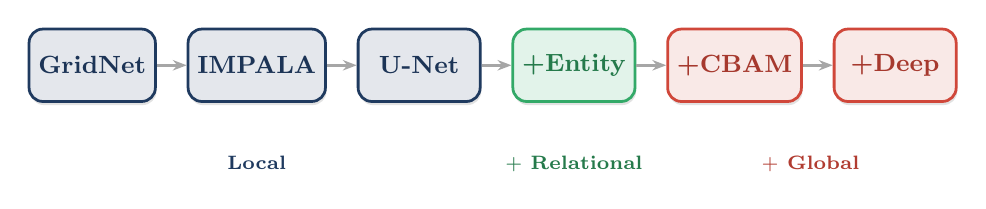
\begin{tikzpicture}[
    pill/.style={rounded corners=5pt, minimum width=1.55cm, minimum height=0.92cm,
      font=\small\bfseries, align=center, line width=1pt,
      drop shadow={shadow xshift=0.4pt, shadow yshift=-1.3pt, opacity=0.25, fill=black!45}},
    loc/.style={pill, draw=uclBlue, fill=uclBlue!12, text=uclBlue!90!black},
    rel/.style={pill, draw=uecdGreen, fill=uecdGreen!14, text=uecdGreen!72!black},
    glo/.style={pill, draw=uecdRed, fill=uecdRed!12, text=uecdRed!80!black},
    arr/.style={-{Stealth[length=5pt]}, black!35, line width=1pt},
    ax/.style={font=\scriptsize\bfseries}]
    \node[loc] (a) {GridNet};
    \node[loc, right=0.38cm of a] (b) {IMPALA};
    \node[loc, right=0.38cm of b] (c) {U-Net};
    \node[rel, right=0.38cm of c] (d) {+Entity};
    \node[glo, right=0.38cm of d] (e) {+CBAM};
    \node[glo, right=0.38cm of e] (f) {+Deep};
    \foreach \x/\y in {a/b,b/c,c/d,d/e,e/f} \draw[arr] (\x)--(\y);
    \node[ax, uclBlue, below=0.55cm of b] {Local};
    \node[ax, uecdGreen!72!black, below=0.55cm of d] {$+$ Relational};
    \node[ax, uecdRed!85!black, below=0.55cm of e, xshift=0.965cm] {$+$ Global};
  \end{tikzpicture}
  \vfill
\end{frame}

\begin{frame}{The UECD architecture}
  \vspace{0.2em}
  \centering
  {\small
    \textbf{\color{black!75}UECD}~$\to$~
    \textcolor{uclBlue}{\bfseries CBAM-gated U-Net} $+$
    \textcolor{uecdGreen}{\bfseries Entity Transformer} $+$
    \textcolor{uecdRed}{\bfseries bottleneck self-attention}\\[0.35em]
    {\footnotesize\color{black!55}$\sim$4.7M params at $C_1{=}48$}\par}
  \vfill
  \fitfig[0.62\textheight]{arch_uecd_simplified_bg.png}
  \vfill
\end{frame}

\begin{frame}{Entity Transformer: relational reasoning}
  \vspace{0.2em}
  \centering
  {\footnotesize\color{black!65}Per-unit tokens attend to all others
    ({\color{uclBlue}\bfseries 2 layers, 4 heads, 128-dim}),\\
    scattered back at {\color{uclBlue}\bfseries two scales}, preserving each unit's identity.\par}
  \vfill
  \fitfig[0.60\textheight]{entity_transformer_simplified_bg.png}
  \vfill
\end{frame}

\begin{frame}{CBAM: attention on what matters}
  \vspace{0.2em}
  \centering
  {\footnotesize\color{black!65}Channel and spatial attention gate each
    residual block: {\color{uclBlue}\bfseries what} features and {\color{uclBlue}\bfseries where}
    on the map (frontlines, exposed units), at {\color{uclBlue}\bfseries negligible cost}
    (under 1\% of each block's weights).\par}
  \vfill
  \fitfig[0.60\textheight]{cbam_resblock_simplified_bg.png}
  \vfill
\end{frame}

\begin{frame}{Global reasoning: seeing the whole map}
  \vspace{0.2em}
  \centering
  {\small\color{black!55}Convolutions are local: even on $16{\times}16$, a unit cannot reach the opposite edge.\\
   The \textbf{\color{uecdRed!80!black}Deep} gives the network a map-wide view.\par}
  \vfill
  \begin{columns}[c]
    \begin{column}{0.46\textwidth}
      \begin{tcolorbox}[enhanced,colback=uecdRed!3,colframe=uecdRed!55,arc=5pt,boxrule=0.8pt,
        title={\faGlobe~~Bottleneck self-attention},coltitle=uecdRed!80!black,colbacktitle=uecdRed!16,
        fonttitle=\small\bfseries,drop fuzzy shadow=black!18,left=9pt,right=9pt,top=8pt,bottom=9pt,
        height=0.47\textheight,valign=center]
        \footnotesize\color{black!72}\raggedright\hyphenpenalty=10000\relax
        Every region attends to every other in a \textbf{single layer}.\\[0.8em]
        Placed at the $H/4\times W/4$ bottleneck:\\
        \textbf{\color{uecdRed!80!black}$256\times$ cheaper} than full resolution.
      \end{tcolorbox}
    \end{column}
    \begin{column}{0.46\textwidth}
      \begin{tcolorbox}[enhanced,colback=uecdRed!3,colframe=uecdRed!55,arc=5pt,boxrule=0.8pt,
        title={\faLayerGroup~~Pyramidal depth},coltitle=uecdRed!80!black,colbacktitle=uecdRed!16,
        fonttitle=\small\bfseries,drop fuzzy shadow=black!18,left=9pt,right=9pt,top=8pt,bottom=9pt,
        height=0.47\textheight,valign=center]
        \footnotesize\color{black!72}\raggedright\hyphenpenalty=10000\relax
        Capacity concentrated at the bottleneck; feeds self-attention and Entity scatter.
        \vspace{1.0em}
        \begin{center}
          
\begin{tikzpicture}[baseline=(current bounding box.center)]
            \foreach \w/\i in {2/0,3/1,4/2,3/3,2/4} {
              \fill[uecdRed!55,rounded corners=0.8pt] (-\w*0.12,\i*0.245) rectangle (\w*0.12,\i*0.245+0.17);}
          \end{tikzpicture}~~~\textbf{\color{uecdRed!80!black}(2, 3, 4, 3, 2)}
        \end{center}
      \end{tcolorbox}
    \end{column}
  \end{columns}
  \vfill
\end{frame}

% =====================================================================
\section{Training Recipe}
% =====================================================================

\begin{frame}{A modular training pipeline}
  \vfill
  \centering
  
\includegraphics[width=\linewidth,height=0.52\textheight,keepaspectratio]{training_pipeline_bg.png}
  \vfill
  \begin{columns}[t]
    \begin{column}{0.32\textwidth}\centering
      {\small{\color{uclAccent}\bfseries 1.}~{\color{uclBlue}\bfseries Fixed PPO baseline}}\\[0.25em]
      {\footnotesize\color{black!55}same hyperparameters; isolates the variable under study}
    \end{column}
    \begin{column}{0.32\textwidth}\centering
      {\small{\color{uclAccent}\bfseries 2.}~{\color{uclBlue}\bfseries Opt-in mechanisms}}\\[0.25em]
      {\footnotesize\color{black!55}each CLI flag-gated, disabled by default}
    \end{column}
    \begin{column}{0.32\textwidth}\centering
      {\small{\color{uclAccent}\bfseries 3.}~{\color{uclBlue}\bfseries Ablated in isolation}}\\[0.25em]
      {\footnotesize\color{black!55}enables the controlled feature ablation}
    \end{column}
  \end{columns}
  \vfill
\end{frame}

\begin{frame}{A catalog of mechanisms, six axes}
  \small
  \vfill
  \begin{columns}[t]
    \begin{column}{0.49\textwidth}
      {\color{uclAccent}\bfseries 1.}~~{\color{uclBlue}\bfseries Action sampling}\newline
      {\scriptsize\color{black!55}$\rightarrow$ autoregressive head, hierarchical sub-action masking}\par\vspace{1.25em}
      {\color{uclAccent}\bfseries 2.}~~{\color{uclBlue}\bfseries Reward \& value signal}\newline
      {\scriptsize\color{black!55}$\rightarrow$ dense-to-sparse scheduling, value heads, PopArt, HL-Gauss, PAE}\par\vspace{1.25em}
      {\color{uclAccent}\bfseries 3.}~~{\color{uclBlue}\bfseries Opponent curriculum \& self-play}\newline
      {\scriptsize\color{black!55}$\rightarrow$ adaptive curriculum, self-play (PFSP), MCW}\par
    \end{column}
    \begin{column}{0.49\textwidth}
      {\color{uclAccent}\bfseries 4.}~~{\color{uclBlue}\bfseries Auxiliary representation}\newline
      {\scriptsize\color{black!55}$\rightarrow$ four shared-encoder heads: ownership, unit count, contrastive, opponent modeling}\par\vspace{1.25em}
      {\color{uclAccent}\bfseries 5.}~~{\color{uclBlue}\bfseries Generalization}\newline
      {\scriptsize\color{black!55}$\rightarrow$ symmetry augmentation, multi-map (PLR)}\par\vspace{1.25em}
      {\color{uclAccent}\bfseries 6.}~~{\color{uclBlue}\bfseries Architecture refinements}\newline
      {\scriptsize\color{black!55}$\rightarrow$ GELU, SPP critic}\par
    \end{column}
  \end{columns}
  \vfill
  \begin{center}{\footnotesize\color{black!55}Around twenty mechanisms, each studied \textbf{\color{uclBlue}one at a time}.}\end{center}
\end{frame}

\begin{frame}{MCW: focus the gradient on close matchups}
  \small\alert{Matchup Competitive Weighting}: a novel, on-policy reweighting inside the PPO update.\par\normalsize
  \vspace{0.6em}
  \begin{columns}[c]
    \begin{column}{0.5\textwidth}
      \small
      \begin{itemize}\setlength\itemsep{0.5em}
        \item Each transition is weighted by how \alert{competitive} its matchup
              is: highest for even ($\sim$50\%) opponents, lowest for
              already-decided ones.
        \item Only the \alert{policy-gradient} term is reweighted; the rollout
              and the value heads stay untouched.
      \end{itemize}
      \vspace{1.0em}
      {\footnotesize\color{black!65}Among the {\color{uclBlue}\bfseries largest gains} in the ablation.}
    \end{column}
    \begin{column}{0.5\textwidth}\centering
      \fitfig[0.66\textheight]{mcw_weight_bg.png}
    \end{column}
  \end{columns}
\end{frame}

% =====================================================================
\section{Results \& Interpretation}
% =====================================================================

\begin{frame}{Architecture ablation: +21.5 pp}
  \centering
  {\small\renewcommand{\arraystretch}{1.0}%
  \begin{tabular}{l r c c c}
    \rowcolor{uclBlue}
    \textcolor{white}{\textbf{Architecture}} & \textcolor{white}{\textbf{Params}} &
    \textcolor{white}{\textbf{Win rate}} & \textcolor{white}{\textbf{Std}} &
    \textcolor{white}{\textbf{$\Delta$ vs GridNet}} \\
    \multicolumn{5}{@{}l}{\scriptsize\itshape\color{uclBlue}Axis 1 \textendash\ Local spatial}\\
    GridNet (baseline)   & 838\,k   & 64.8\% & {\color{black!55}$\pm$3.8} & --- \\
    IMPALA-CNN           & 1.02\,M  & 68.7\% & {\color{black!55}$\pm$5.8} & \textcolor{uecdGreen}{+3.9 pp} \\
    U-Net                & 2.59\,M  & 77.0\% & {\color{black!55}$\pm$1.6} & \textcolor{uecdGreen}{+12.2 pp} \\
    \multicolumn{5}{@{}l}{\scriptsize\itshape\color{hlTeal}Axis 2 \textendash\ Long-range relational}\\
    IMPALA-CNN-Entity    & 1.37\,M  & 74.9\% & {\color{black!55}$\pm$1.2} & \textcolor{uecdGreen}{+10.1 pp} \\
    U-Net-Entity         & 2.90\,M  & 82.7\% & {\color{black!55}$\pm$4.7} & \textcolor{uecdGreen}{+17.9 pp} \\
    U-Net-Entity-CBAM    & 2.90\,M  & 79.1\% & {\color{black!55}$\pm$7.2} & \textcolor{uecdGreen}{+14.3 pp} \\
    \multicolumn{5}{@{}l}{\scriptsize\itshape\color{uclAccent}Axis 3 \textendash\ Global spatial}\\
    \rowcolor{uclAccent!18}
    \textbf{UECD}        & \textbf{4.72\,M} & \textbf{86.3\%} & {\color{black!55}$\pm$7.1} & \textbf{+21.5 pp} \\
    \bottomrule
  \end{tabular}}
  \par\smallskip
  {\footnotesize 7 architectures $\times$ 3 seeds, 100M steps each ($13.6$ GPU-days); grouped by reasoning axis.}
\end{frame}

\begin{frame}{Feature ablation: signal beats capacity}
  \vspace{0.1em}
  \centering
  {\footnotesize\color{black!55}The four reliable gains change \textbf{\color{uclBlue}perception} and \textbf{\color{uclBlue}gradient allocation}, not capacity ($+0.78\%$ params).\par}
  \vspace{0.35em}
  
\includegraphics[width=\linewidth,height=0.78\textheight,keepaspectratio]{feat_ablation_full.png}\\[0.15em]
  {\scriptsize\color{black!50}21 features $\times$ 3 seeds, 50M steps each $\cdot$ 19.4 GPU-days.}
\end{frame}

\begin{frame}{Single-map agent: a discount-induced rush collapse}
  \begin{columns}[c]
    \begin{column}{0.57\textwidth}
      \fitfig[0.82\textheight]{rush_collapse_bg.png}
    \end{column}
    \begin{column}{0.43\textwidth}
      \small
      \begin{itemize}\setlength\itemsep{5pt}
        \item \alert{Setup}: UECD $+$ top-5 scaled to \alert{300M steps}, the
              shaped reward \alert{annealed to sparse} ($1.0\to0$), with self-play.
        \item Once shaped $\to0$ and $\gamma < 1$, the only way to grow return is
              a \alert{shorter episode}.
        \item 750 $\to$ 300 frames amplifies the terminal signal
              \alert{$\sim$92$\times$}: collapse to a worker-rush exploit.
      \end{itemize}
      \vspace{0.5em}
      \begin{tcolorbox}[enhanced,colback=mStandout,colframe=mStandout,arc=4pt,boxrule=0pt,
        left=8pt,right=8pt,top=5pt,bottom=5pt,drop fuzzy shadow=black!25]
        {\footnotesize\color{white}\faWrench~~\textbf{Fix}: a 10\% shaped-reward floor.}
      \end{tcolorbox}
    \end{column}
  \end{columns}
\end{frame}

\begin{frame}{Why it collapses: a discount-induced shortcut}
  \small
  Annealing kills the shaped sum; only the discounted terminal reward survives:
  \[ J(\pi)\;\xrightarrow{\,w_{\text{shape}}\to0\,}\;
     w_{\text{term}}\,\mathbb{E}_{\tau\sim\pi}\!\big[\gamma^{T-1}\,r^{\text{term}}_T\big]
     \;\approx\; 10\,\mathbb{E}_{\tau\sim\pi}\!\big[\gamma^{T-1}\big]. \]
  With $\gamma<1$, $\gamma^{T-1}$ strictly decreases in $T$: the only way to grow
  $J$ is a \alert{shorter episode}, irrespective of play quality.
  \vspace{0.25cm}

  \textbf{It reaches the policy through the advantage}, and the clip fails to
  suppress it.\\
  Two rollouts share $s_t$ but end at $T$ and $T-\Delta$ (same
  state-only $V(s_t)$):
  \[ \hat{A}_t^{(T-\Delta)}-\hat{A}_t^{(T)}
     \;=\;\big(\gamma^{-\Delta}-1\big)\,G_t^{(T)}\;>\;0. \]
  The shorter rollout always gets the larger advantage;\\
  PPO clips the ratio $\rho_t$, \alert{not} $\hat{A}_t$, so the gradient flows.
\end{frame}

\begin{frame}{Rush fragility on held-out opponents}
  \vspace{0.1em}
  \centering
  {\footnotesize\color{black!55}On held-out opponents the rush policy collapses while the balanced one holds:
  the rush is a \textbf{\color{uclBlue}training-distribution exploit}, not transferable.\par}
  \vfill
  \fitfig[0.80\textheight]{rush_fragility_bg.png}
  \vfill
\end{frame}

\begin{frame}{UECD-Best: two-phase fine-tuning}
  \small
  Resume from the \alert{150M (pre-collapse) checkpoint} and fine-tune in two
  short phases, keeping the 10\% shaped floor:
  \begin{itemize}\setlength\itemsep{2pt}
    \item \alert{Phase 1} ($150\text{M}\to240\text{M}$): \alert{broaden the pool}
          --- swap the 3 weakest bots for TMA $+$ ObiBotKenobi, more self-play.
    \item \alert{Phase 2} ($240\text{M}\to350\text{M}$): \alert{harden} ---
          add RAISocketAI to the opponent pool.
  \end{itemize}
  \vspace{0.25cm}
  \centering
  {\footnotesize\renewcommand{\arraystretch}{1.12}%
  \begin{tabular}{l c c c}
    \rowcolor{uclBlue}
    \textcolor{white}{\textbf{Phase}} & \textcolor{white}{\textbf{Steps (M)}} &
    \textcolor{white}{\textbf{On-path}} & \textcolor{white}{\textbf{Full run}} \\
    From scratch              & 0--150   & 34.0 h  & 68.5 h \\
    Phase 1 (broaden pool)    & 150--240 & 30.3 h  & 50.0 h \\
    Phase 2 (vs RAISocketAI)  & 240--350 & 108.7 h & 108.7 h \\
    \rowcolor{uclAccent!18}
    \textbf{Total $=$ UECD-Best} & \textbf{350} & \textbf{7.21 days} & \textbf{9.47 days} \\
    \bottomrule
  \end{tabular}}
\end{frame}

\begin{frame}{Tournament: UECD-Best tops the field}
  \fitfig[0.66\textheight]{final_standings_bg.png}
  \begin{center}\small
    19-agent round-robin on basesWorkers16x16A: \alert{96.67\%} win rate,
    \alert{first of 19}.
  \end{center}
\end{frame}

\begin{frame}{Tournament: the head-to-head matrix}
  \begin{columns}[c]
    \begin{column}{0.55\textwidth}
      \fitfig[0.72\textheight]{h2h_matrix_bg.png}
    \end{column}
    \begin{column}{0.45\textwidth}
      \small
      \begin{itemize}\setlength\itemsep{4pt}
        \item UECD-Best wins \alert{100\%} against every agent but two:
              WorkerRush (50\%) and RAISocketAI (90\%).
        \item This matrix is the CoG protocol: \alert{10 games/matchup},
              \alert{deterministic actions} (not sampling). WorkerRush's 50\% is
              a 2-replay artifact.
        \item Re-run with \alert{sampling} (1000 games): WorkerRush 99.3\%,
              RAISocketAI \alert{65.7\%} ($\pm$2.9). The deterministic 90\% is
              optimistic.
      \end{itemize}
    \end{column}
  \end{columns}
\end{frame}

\begin{frame}{Beyond win rate: Copeland and Nash}
  \begin{columns}[c]
    \begin{column}{0.5\textwidth}\centering
      
\includegraphics[width=\linewidth,height=0.6\textheight,keepaspectratio]{copeland_scores_bg.png}\\[0.25em]
      {\footnotesize \textcolor{uclBlue}{\textbf{Copeland}} (1st, $+17$): breadth ---
      \alert{how many} opponents you beat, regardless of margin.}
    \end{column}
    \begin{column}{0.5\textwidth}\centering
      
\includegraphics[width=\linewidth,height=0.6\textheight,keepaspectratio]{nash_scores_bg.png}\\[0.25em]
      {\footnotesize \textcolor{uclBlue}{\textbf{Nash}} (in support):
      \alert{non-exploitable} vs the equilibrium mix; immune to padding the pool.}
    \end{column}
  \end{columns}
\end{frame}

\begin{frame}{Beyond win rate: $\alpha$-Rank}
  \centering
  \vfill
  
\includegraphics[width=\linewidth,height=0.64\textheight,keepaspectratio]{alpha_rank_sweep_bg.png}\\[0.45em]
  {\footnotesize \textcolor{uclBlue}{\textbf{$\alpha$-Rank}} (1st):
  \alert{evolutionary stability} --- the strategy hardest to invade and displace.}
  \vfill
\end{frame}

\begin{frame}{Beyond win rate: regret}
  \centering
  \vfill
  
\includegraphics[width=\linewidth,height=0.64\textheight,keepaspectratio]{robustness_score_bg.png}\\[0.45em]
  {\footnotesize \textcolor{uclBlue}{\textbf{Regret}} (1st avg, 2nd worst-case):
  \alert{robustness} --- the gap to the pool's best counter for each opponent.}
  \vfill
\end{frame}

\begin{frame}{Generalization: two distribution-shift probes}
  \centering
  {\small Trained \alert{only} on basesWorkers16x16A, then evaluated under two shifts:}\\[0.35cm]
  \begin{tikzpicture}[
    mapnode/.style={inner sep=0pt, line width=1.4pt, sharp corners},
    arr/.style={-{Stealth[length=8pt,width=7pt]}, line width=1.5pt, draw=black!40},
    arrlbl/.style={font=\footnotesize\itshape, text=black!55, inner sep=2pt}]
    \node[mapnode, draw=black!45] (train) at (0,0) {
\includegraphics[height=2.8cm]{map_bw16x16}};
    \node[mapnode, draw=uclBlue] (scale) at (6,1.55) {
\includegraphics[height=2.4cm]{map_bw32x32}};
    \node[mapnode, draw=uecdRed] (layout) at (6,-1.55) {
\includegraphics[height=2.4cm]{map_2bb16x16}};
    \draw[arr] (train.east) -- node[arrlbl,above,sloped,pos=0.5]{larger grid} (scale.west);
    \draw[arr] (train.east) -- node[arrlbl,below,sloped,pos=0.5]{new topology} (layout.west);
    \node[anchor=west, align=left, font=\small] at ([xshift=6pt]scale.east)
      {\bfseries\textcolor{uclBlue}{Scale shift}\\[1pt]{\scriptsize\color{black!55}basesWorkers32x32A}};
    \node[anchor=west, align=left, font=\small] at ([xshift=6pt]layout.east)
      {\bfseries\textcolor{uecdRed}{Layout shift}\\[1pt]{\scriptsize\color{black!55}TwoBasesBarracks16x16}};
  \end{tikzpicture}\\[0.35cm]
  {\footnotesize 100 stochastic-sampling games against 8 opponents on each map.}
\end{frame}

\begin{frame}{Generalization: scale vs layout}
  \begin{columns}[c]
    \begin{column}{0.62\textwidth}\centering
      
\includegraphics[width=\linewidth,height=0.76\textheight,keepaspectratio]{generalization_probes_bg.png}
    \end{column}
    \begin{column}{0.36\textwidth}
      \small
      Tolerates a \alert{scale} shift (32x32), but is brittle under a \alert{layout} shift.\\[0.8em]
      Single-map training overfits \alert{topology} more than \alert{size}.
    \end{column}
  \end{columns}
\end{frame}

\begin{frame}{The five-map training pool}
  \centering
  {\small \alert{UECD-MultiMap} trains on the five open layouts of size
   $\leq 16{\times}16$, shown here \alert{to scale}:}\\[0.5cm]
  {\setlength{\fboxsep}{0pt}\setlength{\fboxrule}{0.8pt}%
  \begin{tabular}{@{}c@{\hspace{0.5cm}}c@{\hspace{0.5cm}}c@{\hspace{0.65cm}}c@{\hspace{0.5cm}}c@{}}
    \fcolorbox{black!40}{white}{
\includegraphics[height=1.4cm]{map_bw8x8}} &
    \fcolorbox{black!40}{white}{
\includegraphics[height=1.4cm]{map_4bw8x8}} &
    \fcolorbox{black!40}{white}{
\includegraphics[height=1.4cm]{map_nwtr9x8}} &
    \fcolorbox{black!40}{white}{
\includegraphics[height=2.8cm]{map_bw16x16}} &
    \fcolorbox{black!40}{white}{
\includegraphics[height=2.8cm]{map_2bb16x16}} \\[0.25em]
    {\scriptsize\bfseries 8x8} & {\scriptsize\bfseries 8x8} & {\scriptsize\bfseries 9x8}
      & {\scriptsize\bfseries 16x16} & {\scriptsize\bfseries 16x16} \\[0.05em]
    {\tiny\color{black!55}basesWorkers8x8A} & {\tiny\color{black!55}FourBasesWorkers8x8}
      & {\tiny\color{black!55}NoWhereToRun9x8} & {\tiny\color{black!55}basesWorkers16x16A}
      & {\tiny\color{black!55}TwoBasesBarracks16x16} \\
  \end{tabular}}
  \\[0.5cm]
  {\footnotesize Three sizes, five topologies. The small boards are almost a
   \alert{different game}:\\
   tiny maps reward an immediate \alert{rush}, unlike the macro play on 16x16.}
\end{frame}

\begin{frame}{Extra experiment \#1: multi-map training}
  \vspace{-2.5mm}
  \begin{tcolorbox}[enhanced, colback=uclBlue!6, colframe=uclBlue!45, boxrule=0.8pt,
      arc=4pt, left=10pt, right=10pt, top=4pt, bottom=4pt, drop fuzzy shadow=uclBlue!12]
    \centering\small
    {\color{uclBlue}\faBullseye}\;{\bfseries\color{uclBlue}GOAL:}\ Can a
    \alert{Prioritized Level Replay (PLR)} curriculum on a \alert{padded environment}\\
    train \emph{one} agent across every map size?
  \end{tcolorbox}
  \vspace{1mm}
  \begin{columns}[T]
    \begin{column}{0.57\textwidth}\centering
      \fitfig[0.62\textheight]{winrates_per_map_bg.png}
    \end{column}
    \begin{column}{0.43\textwidth}
      \footnotesize
      \begin{itemize}\setlength\itemsep{3pt}\setlength\leftmargini{1.1em}
        \item \alert{UECD-SingleMap collapses on 8x8} (14th/16) - yet 8x8 is
              only a \alert{scale} shift the probes called tolerable.
        \item Why: tiny maps reward an immediate \alert{rush}, a strategy
              padding cannot transfer.
        \item \alert{UECD-MultiMap} removes the per-map collapse.
        \item Trade: \alert{82 pts (7th)} vs 141 (1st) at home.
      \end{itemize}
    \end{column}
  \end{columns}
\end{frame}

\begin{frame}{Multi-map: the pipeline works}
  \begin{columns}[T]
    \begin{column}{0.6\textwidth}\centering
      \fitfig[0.76\textheight]{h2h_matrix_global_bg.png}
    \end{column}
    \begin{column}{0.4\textwidth}
      \footnotesize
      \begin{itemize}\setlength\itemsep{4pt}\setlength\leftmargini{1.1em}
        \item Head-to-head, \alert{UECD-MultiMap} beats the specialist
              \alert{UECD-SingleMap} on nearly every matchup.
        \item Trails only on \alert{RAISocketAI} and \alert{ObiBotKenobi}:
              the single-map peak still scores higher.
        \item Only \alert{200M steps / 5 maps}; more budget should flip
              even those two.
      \end{itemize}
      \vspace{4pt}
      \begin{tcolorbox}[enhanced, colback=mStandout, colframe=mStandout, coltext=white,
          arc=3pt, boxrule=0pt, left=8pt, right=8pt, top=5pt, bottom=5pt,
          drop fuzzy shadow=black!25]
        \raggedright
        {\color{uclAccent}\faCheckCircle}\ {\bfseries The \alert{PLR + padding} pipeline
        works: a multi-map agent is feasible.}
      \end{tcolorbox}
    \end{column}
  \end{columns}
\end{frame}

\begin{frame}{Extra experiment \#2: behaviour-cloning warm-start}
  \begin{columns}[c]
    \begin{column}{0.54\textwidth}\centering
      \fitfig[0.54\textheight]{bc_vs_scratch_overall_bg.png}\\[1mm]
      {\scriptsize\color{black!55}Warm-start: BC+VF on \alert{300 bot games}
       ($\sim$313k transitions) vs RAISocketAI, CoacAI, Mayari.}
    \end{column}
    \begin{column}{0.46\textwidth}
      \footnotesize
      Two hypotheses (100M steps):\\[4pt]
      \begin{tcolorbox}[enhanced, colback=uecdGreen!7, colframe=uecdGreen!50, boxrule=0pt,
          borderline west={3pt}{0pt}{uecdGreen}, arc=2pt, left=8pt, right=6pt, top=4pt, bottom=4pt]
        {\bfseries H1. BC speeds up early PPO?}\ \,{\color{uecdGreen}\faCheckCircle\ \bfseries Yes}\\[1pt]
        88\% vs 28\% at 30M; \alert{+41 pp} avg over the first 50M (BC-only already 78\%).
      \end{tcolorbox}
      \vspace{5pt}
      \begin{tcolorbox}[enhanced, colback=uclAccent!7, colframe=uclAccent!50, boxrule=0pt,
          borderline west={3pt}{0pt}{uclAccent}, arc=2pt, left=8pt, right=6pt, top=4pt, bottom=4pt]
        {\bfseries H2. Higher final ceiling?}\ \,{\color{uclAccent}\faMinusCircle\ \bfseries Inconclusive}\\[1pt]
        96\% vs 94\% at 100M, within $\pm$6 pp noise; both plateau at 84--96\%.
      \end{tcolorbox}
    \end{column}
  \end{columns}
  \vspace{0.5mm}
  \begin{tcolorbox}[enhanced, colback=mStandout, colframe=mStandout, coltext=white,
      arc=4pt, boxrule=0pt, left=14pt, right=14pt, top=6pt, bottom=6pt,
      drop fuzzy shadow=black!30]
    \centering\small
    {\color{uclAccent}\faBolt}\hspace{8pt}%
    BC-PPO buys \alert{compute-efficiency}, not a higher plateau:\\
    a much stronger agent \alert{sooner} under a tight budget.
  \end{tcolorbox}
\end{frame}

% =====================================================================
\section{Discussion \& Conclusion}
% =====================================================================

\begin{frame}{Discussion: results vs the literature}
  \begin{columns}[T]
    \begin{column}{0.5\textwidth}
      {\bfseries\color{uclBlue}Where I differ}\\[3pt]
      \begin{itemize}\small\setlength\itemsep{5pt}
        \item \alert{Signal beats capacity}: the reliable gains reshape
              perception and gradient, at near-zero parameter cost.
        \item \alert{BC} speeds up early PPO but lifts no ceiling on a single
              map (vs RAISocketAI's multi-map 72\%$\to$88\%).
        \item The \alert{rush collapse} has no MicroRTS precedent: formalized,
              quantified ($\sim$92$\times$), and mitigated.
      \end{itemize}
    \end{column}
    \begin{column}{0.5\textwidth}
      {\bfseries\color{uclBlue}Where I confirm}\\[3pt]
      \begin{itemize}\small\setlength\itemsep{5pt}
        \item \alert{Relational attention} helps multi-unit control, as in
              StarCraft~II agents.
        \item Single-map training \alert{overfits topology} more than scale.
        \item \alert{Multi-metric} evaluation surfaces structure a plain win
              rate hides.
      \end{itemize}
    \end{column}
  \end{columns}
\end{frame}

\begin{frame}{Honest limitations}
  \begin{columns}[T]
    \begin{column}{0.5\textwidth}
      {\bfseries\color{uclBlue}Deliberate scope}\\[3pt]
      \begin{itemize}\small\setlength\itemsep{5pt}
        \item MicroRTS, not a commercial RTS.
        \item Full observability (no fog-of-war).
        \item Pure RL: no planner, search, or LLM.
        \item Final agent is \alert{single-map}; headline from a single run
              (no seed band).
      \end{itemize}
    \end{column}
    \begin{column}{0.5\textwidth}
      {\bfseries\color{uclBlue}Open gaps}\\[3pt]
      \begin{itemize}\small\setlength\itemsep{5pt}
        \item A monotone \alert{Ranged-only} strategy (narrow RAISocketAI
              margin).
        \item \alert{Topology-shift collapse}: a new layout hurts far more
              than a larger size.
        \item Multi-map agent not yet \alert{competition-grade}.
      \end{itemize}
    \end{column}
  \end{columns}
\end{frame}

\begin{frame}{Future work: four directions}
  \vspace{0.1cm}
  \begin{columns}[T]
    \begin{column}{0.5\textwidth}
      {\linespread{0.9}\selectfont
      \begin{tabular}{@{}c@{\hspace{0.32cm}}m{0.80\linewidth}@{}}
        \contrib{\faComments}{1}{Hybrid DRL + LLM}{LLM plans and models opponents; the 2026 competition pivoted to LLM agents.}\\[2.7em]
        \contrib{\faSitemap}{2}{Hierarchical policy}{Slow strategic tick over per-unit micro-policies.}\\
      \end{tabular}}
    \end{column}
    \begin{column}{0.5\textwidth}
      {\linespread{0.9}\selectfont
      \begin{tabular}{@{}c@{\hspace{0.32cm}}m{0.80\linewidth}@{}}
        \contrib{\faBrain}{3}{Neuro-symbolic}{Compact rules induced from replays gate the policy.}\\[2.7em]
        \contrib{\faDna}{4}{Adversarial PCG}{A regret-based map generator co-evolves with the agent.}\\
      \end{tabular}}
    \end{column}
  \end{columns}
  \vfill
  {\color{uclBlue!18}\hrule height 0.8pt}
  \vspace{0.4em}
  {\centering\footnotesize Each \alert{prototypes on the existing codebase} and closes a named limitation.\\
  The long-term vision targets a \alert{``Ludii for RTS''} with shared transfer protocols.\par}
\end{frame}

\begin{frame}{Conclusion}
  \vfill
  \begin{tcolorbox}[enhanced,colback=uclBlue!5,colframe=uclBlue!30,arc=4pt,
    boxrule=0.7pt,left=12pt,right=12pt,top=8pt,bottom=8pt]
    {\large\color{uclBlue}\faCogs~~\textbf{RQ1}}\quad\rqtag{Design}\\[0.4em]
    The biggest, most \alert{robust} gains come from \alert{perception} (extended
    obs, masks), \alert{competitive self-play} (MCW), and a \alert{relational +
    multi-scale} architecture (\alert{UECD}).
  \end{tcolorbox}
  \medskip
  \begin{tcolorbox}[enhanced,colback=uclBlue!5,colframe=uclBlue!30,arc=4pt,
    boxrule=0.7pt,left=12pt,right=12pt,top=8pt,bottom=8pt]
    {\large\color{uclBlue}\faMicrochip~~\textbf{RQ2}}\quad\rqtag{Budget}\\[0.4em]
    \alert{Yes}: UECD-Best surpasses RAISocketAI on a fixed layout at
    $\sim$9.5 GPU-days, at the cost of cross-layout robustness.
  \end{tcolorbox}
  \vfill
  {\centering\footnotesize An \alert{open-source pipeline}: a substrate for future
   hybrid DRL/LLM MicroRTS agents.\par}
\end{frame}

% --- Image credits: slide / description / source table (before the Thank-you) ---
{\setbeamertemplate{footline}{}%
\begin{frame}[noframenumbering]{Image credits}
  \centering
  \vspace{0.55cm}
  {\footnotesize\renewcommand{\arraystretch}{1.5}%
  \setlength{\tabcolsep}{10pt}%
  \begin{tabular}{@{}>{\centering\arraybackslash}m{1.1cm} l l@{}}
    \rowcolor{uclBlue}
    \textcolor{white}{\textbf{Slide}} & \textcolor{white}{\textbf{Figure}} & \textcolor{white}{\textbf{Source}} \\
    1  & StarCraft~II screenshot      & \href{https://starcraft2.blizzard.com}{\color{uclBlue}Blizzard Entertainment (2010)} \\
    1  & Warcraft~III screenshot      & \href{https://warcraft3.blizzard.com}{\color{uclBlue}Blizzard Entertainment (2002)} \\
    3  & MicroRTS game state          & \href{https://onlinelibrary.wiley.com/doi/10.1609/aimag.v39i1.2777}{\color{uclBlue}Onta\~n\'on et al., \emph{AI Magazine} (2018)} \\
    6  & Agent--environment loop      & \href{http://incompleteideas.net/book/the-book-2nd.html}{\color{uclBlue}Sutton \& Barto, \emph{RL: An Introduction} (2018)} \\
    14 & AlphaStar architecture       & \href{https://www.nature.com/articles/s41586-019-1724-z}{\color{uclBlue}Vinyals et al., \emph{Nature} (2019)} \\
    \textit{all} & Interface icons     & \href{https://fontawesome.com}{\color{uclBlue}Font Awesome 5 Free (CC BY 4.0)} \\
  \end{tabular}}
  \vspace{0.65cm}\par
  {\footnotesize\itshape\color{black!50}All other figures and diagrams are the author's own work. All sources are clickable.\par}
\end{frame}}

{\setbeamertemplate{footline}{}%
\setbeamercolor{background canvas}{bg=mStandout}%
\begin{frame}[plain,noframenumbering]
  \color{white}\centering
  \settowidth{\thankwidth}{\fontsize{50}{54}\selectfont\bfseries Thank you}%
  \vfill
  {\fontsize{50}{54}\selectfont\bfseries Thank you\par}
  \vspace{0.25em}
  {\fontsize{22}{26}\selectfont\color{white!70}Questions?\par}
  \vspace{0.5cm}
  {\color{hlTeal}\fontsize{9}{9}\selectfont
   \makebox[\thankwidth]{%
     \faRobot\hfill\rule[2.2pt]{0.5cm}{0.7pt}\hfill\faRobot\hfill\rule[2.2pt]{0.5cm}{0.7pt}\hfill
     \faRobot\hfill\rule[2.2pt]{0.5cm}{0.7pt}\hfill\faRobot\hfill\rule[2.2pt]{0.5cm}{0.7pt}\hfill
     \faRobot\hfill\rule[2.2pt]{0.5cm}{0.7pt}\hfill\faRobot\hfill\rule[2.2pt]{0.5cm}{0.7pt}\hfill\faRobot}\par}
  \vspace{0.5cm}
  {\footnotesize%
  \renewcommand{\arraystretch}{1.35}%
  \begin{tabular}{@{}r@{\hspace{0.5cm}}l@{}}
    {\color{hlTeal}\faEnvelope} & \href{mailto:mathis.delsart@gmail.com}{\color{white!60}mathis.delsart@gmail.com}\\
    {\color{hlTeal}\faGithub} & \href{https://github.com/mathisdelsart/microrts-drl-uecd}{\color{white!60}github.com/mathisdelsart/microrts-drl-uecd}\\
    {\color{hlTeal}\faGlobe} & \href{https://mathisdelsart.github.io/microrts-drl-uecd-website}{\color{white!60}mathisdelsart.github.io/microrts-drl-uecd-website}\\
  \end{tabular}\par}
  \vfill
\end{frame}}

\end{document}
